\newpage
\section{Modelli linari}
\subsection{Regression}
Un possibile esempio di regressione potrebbe essere un processo di stima di una funzione di valore
reale sulla base di un insieme finito di campioni rumorosi. Le conoscenze sarebbero $pairs(x, f(x) + random noise)$.\\
La task a questo punto sarebbe trovare $f$ per i dati nella seguente tabella.
\begin{figure}[h!]
    \centering
    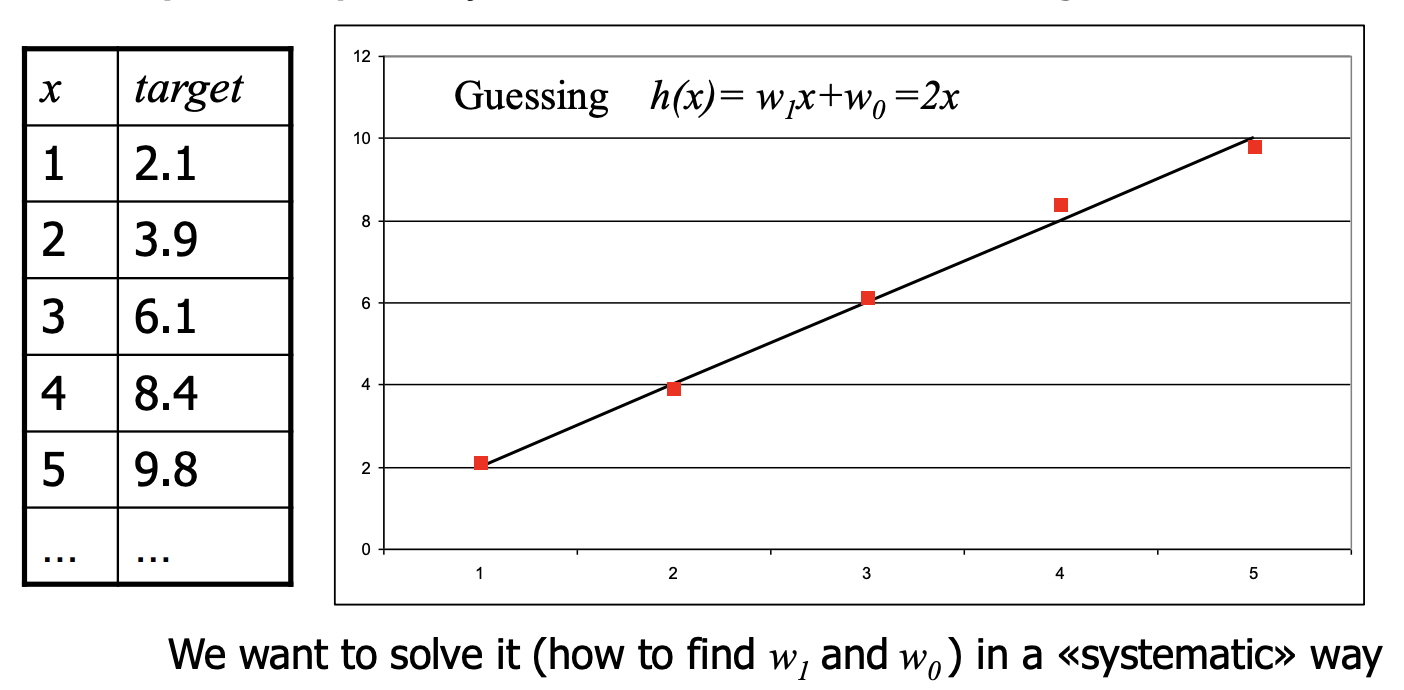
\includegraphics[width=0.65\textwidth]{images/esempio-regresione.png}
\end{figure}
\begin{example}
    Esempio di modelli linari:
    \begin{figure}[h!]
        \centering
        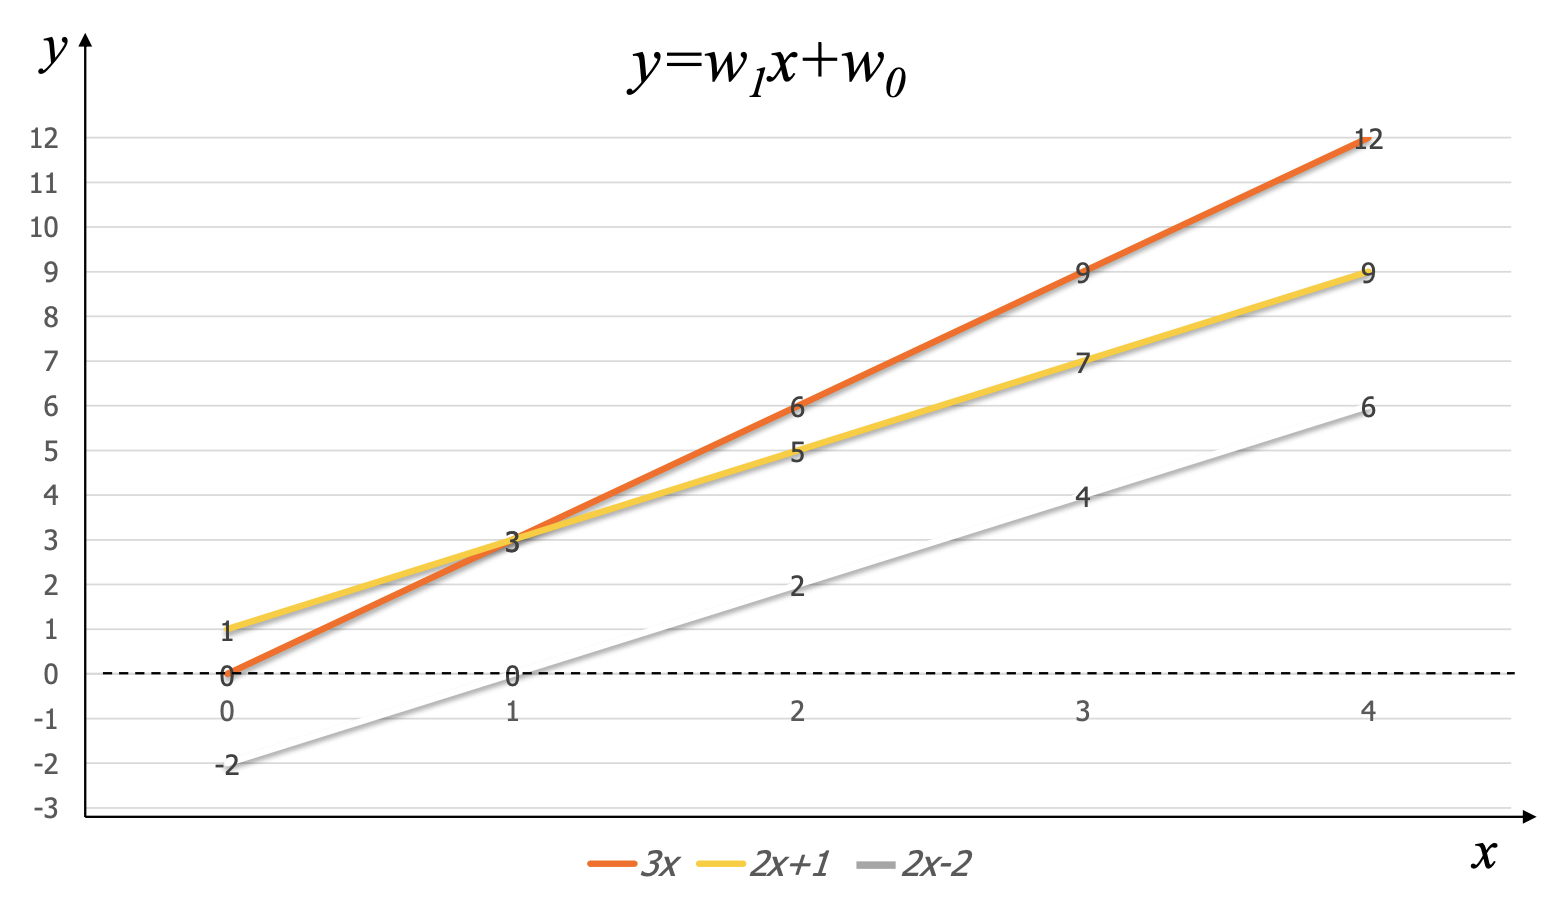
\includegraphics[width=0.65\textwidth]{images/esempio-modelli-lineari.png}
    \end{figure}
\end{example}

\subsubsection{Univariate linear regression}
Il caso univariante, semplice regressione linieare: iniziamo con 1 valore di inputl, $x$ e 
1 valore di output $y$.
\begin{definition}
    Assumiamo che un modello $h_w(x)$ espresso come:
    $$out = h(x) = w_1x + w_0$$
    dove $w$ è il coefficiente a valore reale/paramentro libero (peso).
\end{definition}
Si cerca di avere un adattamento dei dati secondo una “linea retta”. Trovare $h$ (modello lineare) che 
meglio si adattano ai dati (da gli insieme di dati osservati dei valori $x$ e $y$). Assumiamo che la variabile data (y) è (linearmente) 
associata ad un'altra viarialbe (x) o più variabili, da $y = w_1x + w_0 + noise$, dove $w$ è il free par e $noise$ è
un errore misurato al target (con una distribuzione normale). Andiamo a costruire un modello (trovare il valore $w$) per predirre/stimare il prezzo ($y$) dei punti
per altri (osservabile) valori $x$ (prediction).
\begin{figure}[h!]
    \centering
    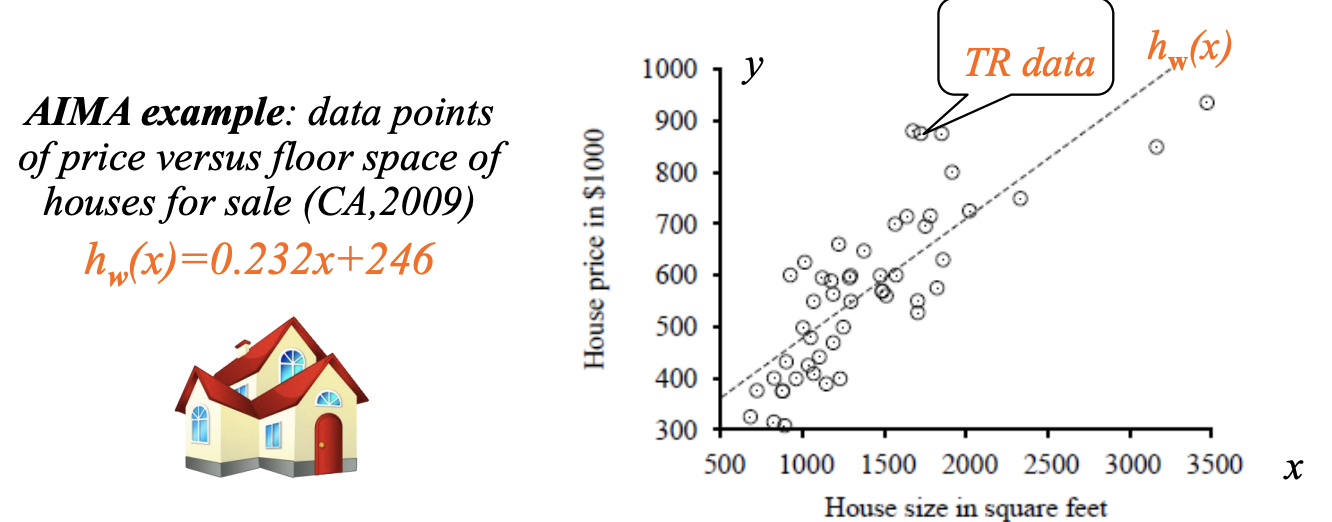
\includegraphics[width=0.55\textwidth]{images/task-model-esempio.png}
\end{figure}
Usiamo poi questi valori per \textbf{predirre/stimare} il prezzo (t) dei punti per altri valore osservabili.
\begin{figure}[h!]
    \centering
    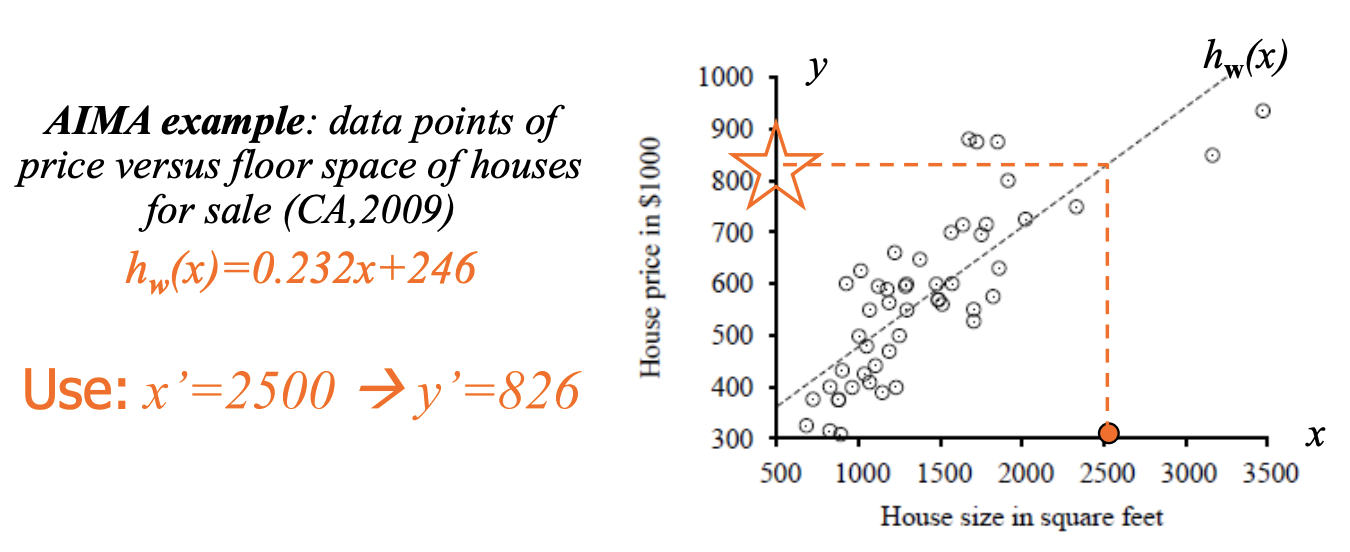
\includegraphics[width=0.55\textwidth]{images/uso-predizione-esempio.png}
\end{figure}

\subsubsection{Learning via LMS}
Abbiamo capito che quindi dobbiamo andare a trovare i valori dei paramentri $w$ ($w_1$ e $w_2$ nei casi univarianti) per andare a minimizzare 
l'output dell'errore del modello (per eseguire un buon fitting). In uno spazio di ipotesi infinito (valore $w$ continuo) abbiamo una buona soluzione
data dalla matematica classica, possiamo "imparare" da dei semplici tools, sebbene semplice incluse moltri concetti rileventi per
il ML moderno ed è alla abse dei metodi evoluti in the field. Definiamo qui una \textbf{funzione less / error} e usiamo il \textbf{Least Mean Square (LMS)} approccio.\\\\
\textbf{Il training} si fa trovando $w$ tale che minimizzi l'\textbf{errore}/la \textbf{perdita epirica} (il miglior dato che fitta nel training set con l'esempio $l$)

\begin{definition}
    Andiamo allora a definire LMS con:
    \begin{itemize}
        \item \textbf{Given} un insieme ti esempi di training $l$ ($x_p, y_p$) $p = 1 \dots l$
        \item \textbf{Trovare} $h_w(x)$ nella forma $w_1 x + w_0$ (quindi i valori di $w$) che minimizzano la perdita attesa dei dati di training.
    \end{itemize}
    Per la perdita usiamo la radice dell'errore.\\
    Da qui il \textbf{least (mean) square} si tratta di trovare la $w$ che minimizzi la somma residua delle ragdici [$argmin_w Error(w) in L_2$]
    $$Loss(h_w) = E(w) = \sum_{p=1}^{l} (y_p - h_w(x_p))^2 = \sum_{p=1}^{l}(y_p - (w_1 x_p + w_0))^2$$
    Dove $x_p$ è $p-th$ input/pattern/esample, $y_p$ l'output per $p$, $w$ free par., $l$ numero degli esempi.
\end{definition}
\hspace{-15pt}Perché usare LMS per adattarsi ai dati con $h$? Il \underline{least (mean) square} trova $w$ per minimizzare la \textbf{somma di radici residua} [$argmin_w Error(w) \in L_2$]:
\begin{figure}[h!]
    \centering
    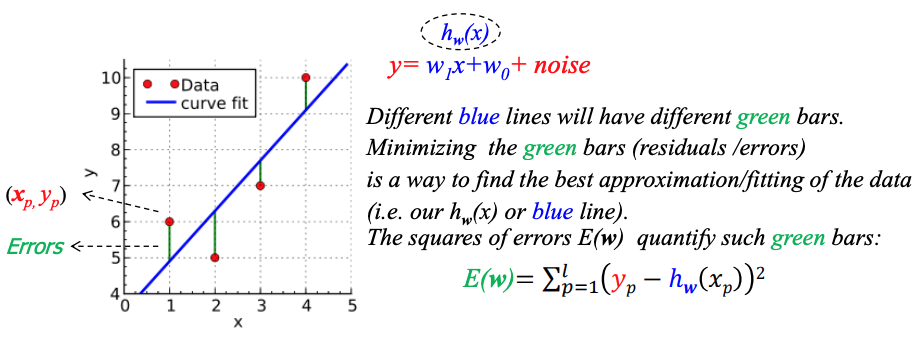
\includegraphics[width=0.6\textwidth]{images/lms.png}
\end{figure}

\hspace{-15pt}Il metodo dei minimi quadrati è un approccio standard alla soluzione approssimata di sistemi sovradeterminati, cioè insiemi di equazioni
in cui ci sono più equazioni che "sconociuti".\\\\
\textbf{Come si risolve?} Ricorda che il minimo locale è un punto stazionario, il gradiente è nullo.
$$\frac{\partial E(wi)}{\partial w_i} = 0 \hspace{15pt} i = 1, \dots, dim\_input + 1$$
Per una semplice regressione lineare (2 paramentri liberi) abbiamo che:
$$\frac{\partial E(w)}{\partial w_0} = 0 \hspace{15pt} \frac{\partial E(w)}{\partial w_1} = 0$$
Funzione di perdita convessa $\Rightarrow$ abbiamo la seguente soluzione (senza minimo locala).
$$w_1 = \frac{\sum x_p y_p - \frac{1}{l}\sum x_p \sum y_p}{\sum x_p^2 - \frac{1}{l} (\sum x_p^2)} = \frac{Conv[x, y]}{Var[x]}, \hspace{10pt} w_0 = \overline{y} - w_1 \overline{x} \hspace{20pt} \overline{y} = \frac{1}{l}\sum_{p \to 1} t_p  \hspace{7pt} \overline{x} = \frac{1}{l}\sum_{p\to 1}x_p$$
Calcolare il gradiante per 1 (ciascuno, omettendo quindi $p$ per $x$) pattern p. 
$$\frac{\partial E}{\partial w_i} = \frac{\partial (y - h_w(x))^2}{\partial w_i} = 2(y - h_w(x))\frac{\partial (y - h_w(h))}{\partial w_i} = 2(y - h_w(x))\frac{\partial (y - (w_1 x + w_0))}{\partial w_i}$$

\subsection{Summarizing}
\begin{itemize}
    \item \textbf{Given} un insieme di $l$ esempi di training ($x_p, y_p$) ed una funzione di perdita.
    \item \textbf{Find} il valore del peso $w$ per costruire $h_w(x)$ espresso come $y/out = w_1 x + w_0$ (minimizzare la perdita attesa dei dati di training)
\end{itemize}
\begin{figure}[h!]
    \centering
    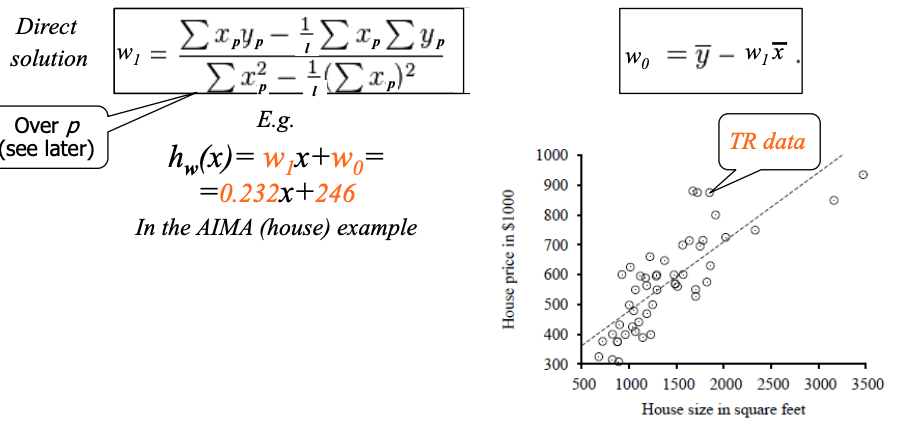
\includegraphics[width=0.55\textwidth]{images/summarizing.png}
\end{figure}
Ora è possibile usarlo per nuovi $x'$ per predirre $y'$. Vediamo ora un approccio differente.

\subsection{Gradiant descent (ricerca locale)}
Errore delle superfici per il linear model con 2 pesi. Parabolico per $E(w) = E([w_0, w_1]^T)$ (funzione quadratica convessa)
\begin{figure}[h!]
    \centering
    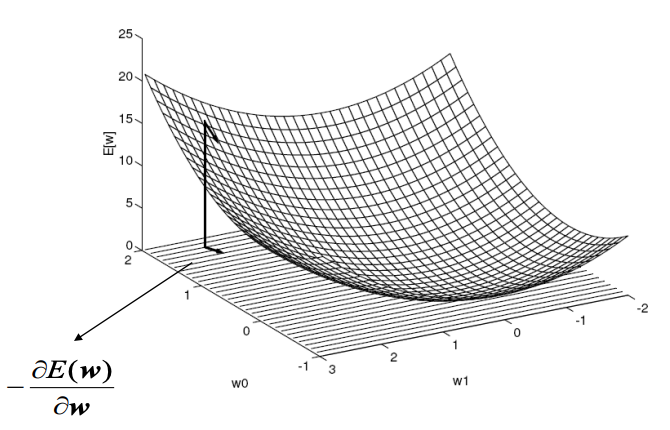
\includegraphics[width=0.4\textwidth]{images/error-surface.png}
\end{figure}

\hspace{-15pt}Spazio ipotetico con 2 parametri $w_0, w_1$. Il gradiente di $E(w)$ è il nostro "compasso" per trovare il minimo.\\\\
La derivazione precedente suggerisce la linea per costruire un \textbf{algoritmo iterativo} basato su $\frac{\partial E(w)}{\partial w_i}$
\begin{definition}
    \textbf{Gradiente} = direzione salita, possiamo muoverci verso il minimo con un gradiente in discesa ($\Delta w =$ gradiente di $E(w)$)
\end{definition}
\begin{definition}
    \textbf{ricerca locale} inizia con vettore di pesi iniziali. Esso viene modificato iterativamente per diminuire
    fino a minimizzare la funzione di errore (discesa più ripida).
    $$w_new = w + \eta \cdot \Delta w$$
    Dove $\eta$ è una constante (step size) chiamata \textbf{learning rate}
\end{definition}
\begin{figure}[h!]
    \centering
    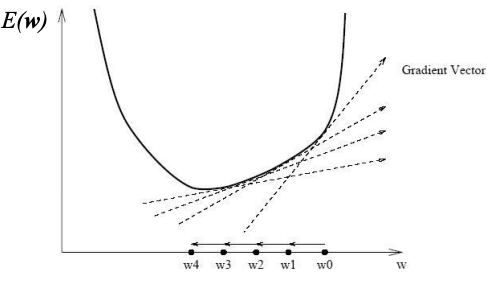
\includegraphics[width=0.5\textwidth]{images/gradieant-descent.png}
\end{figure}
Le motivazioni intuitive del gradiant descent sono che dalla formulazione, $w_new = w + \eta \cdot \Delta w$ possiamo ottenere:
$$\Delta w_0 = -\frac{\partial E(w)}{\partial w_0} = 2(y- h_w(x)) \hspace{15pt} \Delta w_1 = -\frac{\partial E(w)}{\partial w_i} = 2(y - h_w(x)) \cdot x$$
\begin{definition}
    Questa è una "error correction rule" chiamata \textbf{delta rule} che cambia la proporzione $w$ con l'errore (target-output):
    \begin{itemize}
        \item (target y - output) = err  = 0 $\to$ nessuna correzione 
        \item output > target $\to$ (y - h) < 0 (output troppo alto)
        \begin{itemize}
            \item Se $\Delta w_0$ negativo $\to$ si riduce $w_0$ e 
            \item if (input $x > 0$) $\Delta w_1$ negativo $\to$ si ricude $w_q$ else si aumenta $w_1$
        \end{itemize}
        \item output < target $\to$ $(y - h) > 0$ (output è troppo lento)
    \end{itemize} 
\end{definition}
\hspace{-15pt}In questo modo andiamo a migliorare l'apprendimento dai precedenti errori.\\\\
In conclusione possiamo dire che l'approccio del Gradiant descent è semplice ed efficacie per ricerca locale e approcci alla soluzione LMS, inoltre
ci permette di cercare in uno spazio infinito di ipotesi, può essere facilmente applicato sempre per $H$ contuno e perdite differenziabili non solo ai modelli lineari
(ess. reti neurali e deep learning models). A livello di efficienza molti miglioramenti sono possibili come il Newton's method, Conjugate Gradiant.

\subsection{Estensioni a $l$ dati}
\begin{definition}
    Possiamo riassumente per $l$ patterns $(x_p, y_p)$ nel seguente modo.
    $$\Delta w_0 = - \frac{\partial E(w)}{\partial w_0} = 2 \sum_{p=1}^{l}(y_p - h_w(x_p)) \hspace{15pt} \Delta w_1 = -\frac{\partial E(w)}{\partial w_1} = 2 \sum_{p=1}^{l}(y_p - h_w(x_p)) \cdot x_p$$
    Dove $x_p$ è un p-esmo input, $y_p$ l'output per $p$, $w$ una coppia libera, $l$ numero di esempi.
\end{definition}
\hspace{-15pt}Possiamo aggiornare $w$ dopo (ripetendo) una fase di dati di training $l$ $\to$ \textbf{algoritmo di batch} (blu). Oppure
possiamo aggiornare $w$ dopo ogni pattern $p \to$ \textbf{on-line algorithm} (discesa del gradiente stocastico) (purple and green), questo caso 
potrebbe essere più veloce, ma necessitare di step più piccoli.

\subsection{Estendere a vettori di input}
Questo è una caso standard, usare da 2 finoa centinaia di variabili/features di input  $x = [x_1, x_2, \cdots, x_n]$, il \textbf{pattern} di input
è un vettore.
\begin{example}
    Degli esempi potrebbero essere calcolare lo stato di una scacchiera in un gioco di dama per num. di pezzi bianchi/neri/re/catturati
    nel turno successivo: 6 variabili. $w$ peso che viene dalle "fetures sul tavolo".
\end{example}
\hspace{-15pt}Facciamo un piccolo riassunto della notazione per i dati. Prendiamo una $X$ matrice $l, x, n$ dove $l$ sono le righe
mentreh $n$ le colonne (feuteres, variabili, attributi), $p = 1, \cdots, l$ e $i = 1, \cdots n$. Abbiamo spesso bisogno di omettere alcuni
indici quando il contesto è chiaro, ad es:
\begin{figure}[h!]
    \centering
    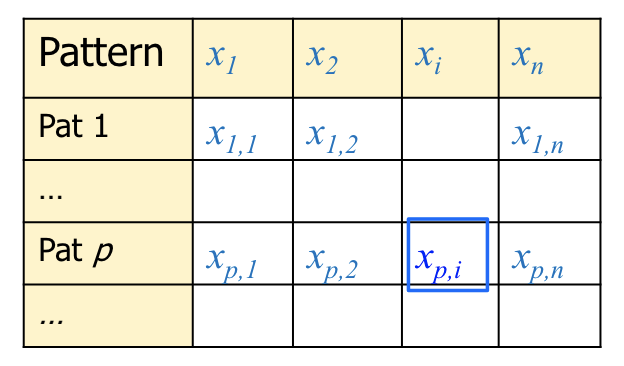
\includegraphics[width=0.5\textwidth]{images/resume-data-notation.png}
\end{figure}
\begin{itemize}
    \item Ogni riga, $x$ generica (vettore in grassetto), un raw nella tabella: (input) esempio, pattern, instance, sample, ..., input vector, ...
    \item $x_i$ o $x_j$ (scalari): componenti $i$ o $j$ (dato un pattern, omettendo p).
    \item $x_p$ (o $x_i$) (vettor in grassetto) il p-esimo (o i-esimo) raw nella tabella = pattern $p$ (o i)
    \item $x_p,i$ (scalare) anche come ($x_p$): componente $i$ nel pattern $p$ (o usamo $x_p,j$ per il componente j, ecc.)
    \item Per il target sono solitamente usiamo solo $y_p$ con $p=1, \cdots l$ (lo stesso per $d$ o $t$)
\end{itemize}
Per la notazione di input multidimensionali andiamo ad assumere una colonna vettere per $x$ e $w$ (in grassetto). Numero 
del dato $l$, dimensione del vettore di input $n$, $y_p$ (targets) e $p = 1, \cdots, l$
$$w^t x + w_0 = w_0 + w_1 x_1 + w_2 x_2 + \cdots w_n x_n = w_0 + \sum_{i=1}^{n} w_i x_i$$
\begin{note}
    Notare che spesso, come prima, la notazione di trasposta $T$ in $w^T$ è omessa.
\end{note}
\hspace{-15pt}$w_0$ è l'intercetta, la soglia, il bias, l'offset.. Spesso è conveninente per includere la constante $x_0 = 1$ 
in modo che possiamo scriverlo come:
$$w^T x = x^T w (inner product) \hspace{15pt}x^T = [1, x_1, x_2, \cdots, x_n] \hspace{15pt} w^t = [w_0, w_1, w_2, \cdots, w_n]$$
\begin{note}
    Notare che $w$ è un parametro (libero) continuo "pesi".
\end{note}
\newpage
\hspace{-15pt}In una vista geometrica avremmo quello che si chiama \textbf{iperpiano}. Per 2 variabili avremmo:
$$x^T w = w^T x = w_0 + w_1 x_1 + w_2 x_2 \hspace{20pt} \text{(n dim)} w^t = [w_0, w_1, w_2, \cdots, w_n]$$
\begin{figure}[h!]
    \centering
    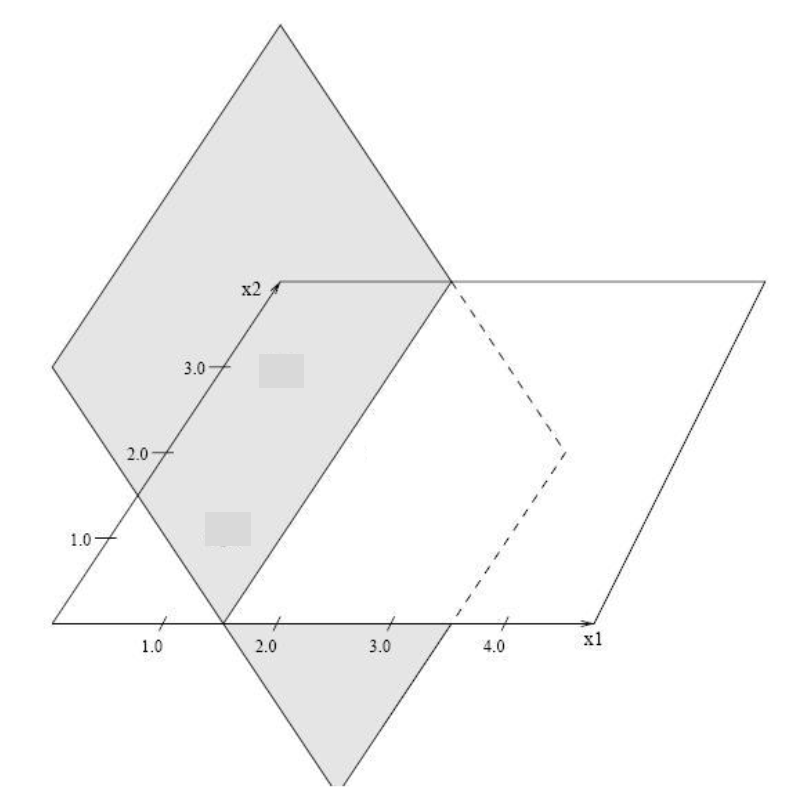
\includegraphics[width=0.2\textwidth]{images/hyperplane.png}
\end{figure}
Quindi possiamo definirlo come:
$$h(x_p) = x_p^T w = \sum_{i=0}^{n}x_{p,i} w_i$$
Possimao sintetizzare il caso con input di dimensione n, e l patterns nel seguenti modo:
\begin{itemize}
    \item \textbf{Given} un insieme di $l$ esempi di trainign $x_p, y_p$
    \item \textbf{Find} il peso del vettore $w$ che minimizzi la perdita attesa dei dati di training.
\end{itemize}
$$E(w) = \sum_{p=1}^{l}(y_p - x_p^T w)^2 = ||y - Xw||^2$$
Dove $x_p$ è il p-esimo input del vettore, $y_p$ è l'outpu per p, $w$ è la coppia libera, $l$ il numero
di esempi e $n$ la dimensione dell'input.

\subsection{Algoritmo iterativo di discesa del gradiante}
\begin{definition}
    Definiamo ora \textbf{l'algoritmo iterativo di discesa del gradiante}
    $$\Delta w_i = -\frac{\partial E(w)}{\partial w_i} = \sum_{p=1}^{l}(y_p - h_w(x_p)) \cdot x_{p,i} = w\sum_{p=1}^{l}(y_p - x_p^T w)x_{p,i}$$
    Abbiamo che il 2 è una costante che può essere ignorata nello sviluppo dell'algoritmo, mentre $x_{p,i}$ è il componente $i$ del pattern $p$
\end{definition}
\hspace{-15pt}Questo è una estensione vettoriale al gradiente molto semplice nel quale ogni x, ha il suo $w_i$ e il suo $\Delta w_i$ (come il singolo x prima).
Il vettore di gradianti per una dimensione n sarebbe il seguente:
$$
\Delta w = -\frac{\partial E(w)}{\partial w} = 
\begin{bmatrix}
    -\frac{\partial E(w)}{\partial w_1}\\
    -\frac{\partial E(w)}{\partial w_2}\\
    -\frac{\partial E(w)}{\partial w_i}\\
    \cdots\\
    -\frac{\partial E(w)}{\partial w_n}
\end{bmatrix}
= 
\begin{bmatrix}
    \Delta w_1\\
    \Delta w_2\\
    \Delta w_i\\
    \cdots \\
    \Delta w_n
\end{bmatrix}
$$
Possiamo lavorare in uno spazio a più luci senza la necessità di visualizzarlo. PS $w_0$ viene omesso sopra, puoi includerlo facilmente.\\\\
Per riassumenre possiamo spiegare l'algorimo in dei semplici passaggi:
\begin{enumerate}
    \item Iniziare con un vettore dei pesi $w_initial$ (piccolo), fissando un $\eta$ ($0 < \eta < 1$).
    \item Calcolare $\Delta w =$ -"gradiante di $E(w)$" = $-\frac{\partial E(w)}{\partial w}$ (o per ogni $w_j$)
    \item Calcolare $w_new = w + \eta \cdot \Delta w$ (o per ogni $w_j$) 
    \item Ritornare al 2 e ripetere finché non si converge o $E(w)$ è "sufficetemente piccolo"
\end{enumerate}
$\Delta w/l$ least mean square:
\begin{itemize}
    \item Batch versions ($\Delta w$ dopo ogni "epoch" dei dati "l")
    \item Stochatic/on-line version: aggiornare w per ogni pattern p (da $\Delta_p w = x_p (y_p - x_p^T w)$ senza aspettare la somma totale su $l$)
    \item $\eta$ = learning rate: seed/stabilty trade-off: può essere (gradualmente) decrementato a zero (garantendo convergenza, 
    evitando oscillazioni intorno al min.)
\end{itemize}
\begin{figure}[h!]
    \centering
    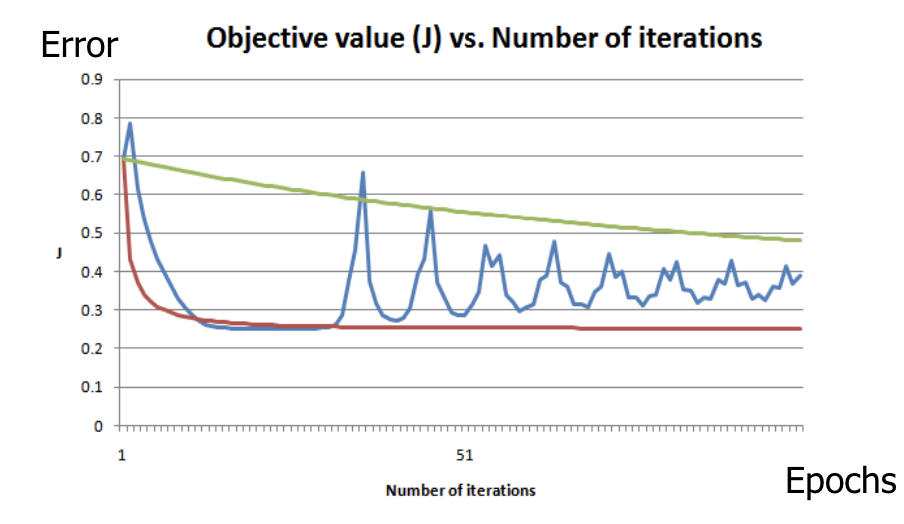
\includegraphics[width=0.6\textwidth]{images/learning-curve-examples.png}
\end{figure}
\begin{definition}
    Queste sono le \textbf{curve di apprendimento}: Mostrano come si verifica l'errore diminuisce attraverso il gradiente iterazioni di discesa.
\end{definition}
I vantaggi dei modelli lineari sono che se funzionano bene sono un modello fantastici: molto semplice,
tutte le informazioni dei dati sono in $w$, facili da interpretare, dati "rumorosi" sono accettati, Fenomeni lineari: un sogno per la scienza: ideale per realizzare un fenomeno “naturale”.
legge.

\subsection{Limitazioni}
Una delle limitazioni dei modelli lineari sono le tasks di regressione per problemi non lineari.
\begin{figure}[h!]
    \centering
    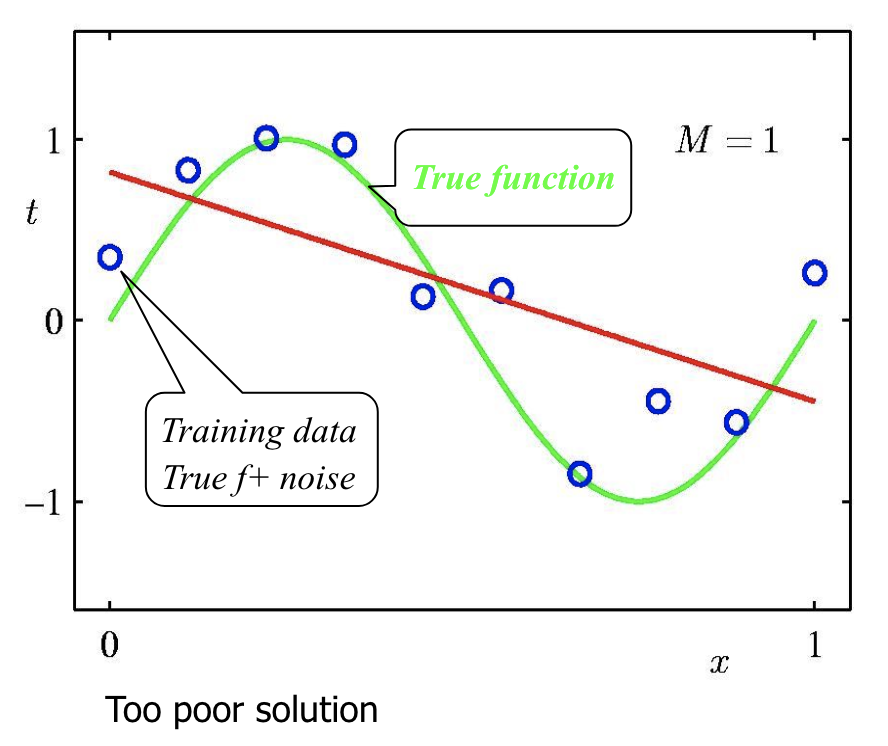
\includegraphics[width=0.3\textwidth]{images/regression-task-non-linear-problems.png}
\end{figure}

\hspace{-15pt}Proviamo ora a muoverci verso delle relazioni non-lineari. Notare che in $h_w(x) = w_1 x + w_0$ o $h_w(x) = w^T \cdot x$ 
come modelli statistici parametrici: "\textbf{lineare}" non si riferisce a questa linea rette, piuttosto al modo in cui
si verificano i coefficienti di regressione $w$ nell'equazione di regressione.\\\\
Possiamo quindi utilizzare anche input trasformati, come ad esempio $x, x^2, x^3, x^4, \cdots$ con una relazione \textbf{non lineare} input e outpout, 
gestiamo la macchina di learning (Least Square solution) sviluppandola nel seguente modo:
$$h_w(x) = w_0 + w_1 x + w_2 x^2 + \cdots + w_Mx^M = \sum_{j=0}^{M}w_j x^j$$
Detta \textbf{polynomial regression}.
\newpage
\begin{example}
    Facciamo un esempio non-lineare.
\end{example}
\begin{wrapfigure}[10]{r}{0.4\textwidth}
    \vspace{-25pt}
    \centering
    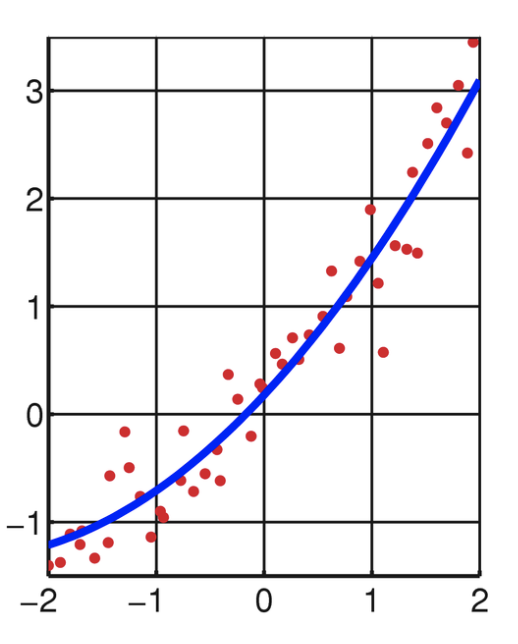
\includegraphics[width=0.2\textwidth]{images/esempio-non-lineare.png}
\end{wrapfigure}
Il risultato dell'adattamento di una funzione quadratica (in blu) $M=2$, passante un insieme di punti dati (in rosso). \\\\
Nei minimi quadrati lineari la dunzione non deve essere lineare in argomento (varibili di input) ma solo nei parametri ($w$) che sono
determinati per dare il best fit.

\subsection{Linear basis expansion}
Una generalizazzione (che mostriamo per la regressione) è la \textbf{LBE} o \textbf{linear basis expansion}, che definiamo come
$$h_w(x) = \sum_{k=0}^{K}w_k\phi_k(x)$$
L'argomento di input è un vettore con variabili aggiuntive, le quali sono trasformazioni di $x$ secondo una funzione $\phi$ ($\phi_k: R^n \to R$).
\begin{example}
    Alcuni eesempi sono:
    \begin{itemize}
        \item Rappresentazione polinomiale $x: \phi(x) = x_j^2$ o $\phi(x) = x_jx_i$ ...
        \item Trasformazione non lineare di un singolo input $\phi(x) = \log(x_k), \phi(x) = root(x)$, ...
        \item Trasformazione non lineare di input multipli: $\phi(x) = ||x||$
        \item Splines, ...
    \end{itemize}
\end{example}
\hspace{-15pt}Il numero di paramentri $K>n$. Il modello è lineare nei paramentri (anche in $\phi$, non in $x$): possiamo usare lo stesso
algorimo di learning di prima.

\begin{example}
    [1-dim $x$] \hspace{15pt} $\phi_j(x) = x^j$.
    $$h(x) = w_0 + w_1x + w_2x^2 + \dots + w_Mx^M = \sum_{j=0}^{M}w_jx^j$$
    1-dim regressione polinomiale ($K=M$). Per il numero di termini nel polinomio con D dim. input vedremo più avanti.\\\\
    O "qualsiasi altro" $\phi(x) = \phi([x_1, x_2, x_3])$
    $$h(x) = w_1x_1 + w_2 x_2 + w_3 \log(x_2) + w_4\log(x_3) + w_5(x_2x_3) + w_0$$
\end{example}
\hspace{-15pt}Vediamo ora le criticità (sia positive che negative) del basis expansion, per poi arrivare 
ai così detti approcci "\textbf{dizionari}".
\begin{itemize}
    \item \textbf{PROS}: È più espressivo: può modellare in modo più complicato
    relazioni (rispetto a quelle lineari).
    \item \textbf{CONS}: Con un'ampia base di funzioni, abbiamo bisogno di metodi per
    controllare la complessità del modello.
\end{itemize}
$$h_w(x) = w_0 + w_1x + w_2x^2 + \dots + w_Mx^M = \sum_{j=0}^{M}w_jx^j$$
\newpage
\begin{figure}[h!]
    \centering
    \begin{subfigure}{.3\textwidth}
        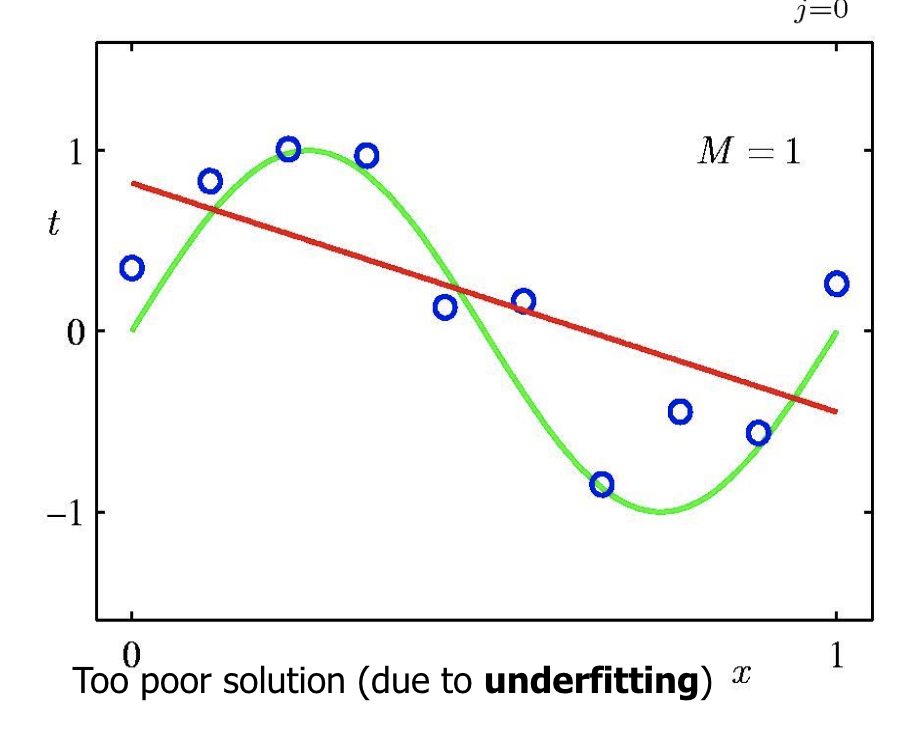
\includegraphics[width=\textwidth]{images/1st-order-polynomial.png}
        \caption{1st order polynomial}
    \end{subfigure}
    \begin{subfigure}{.3\textwidth}
        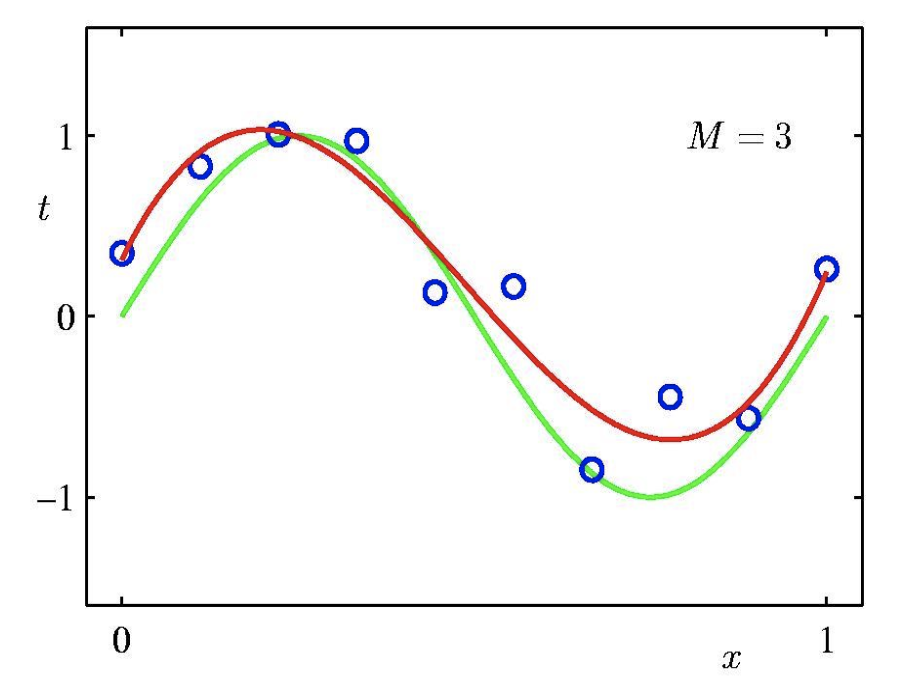
\includegraphics[width=\textwidth]{images/3st-order-polynomial.png}
        \caption{3st order polynomial}
    \end{subfigure}
    \begin{subfigure}{.3\textwidth}
        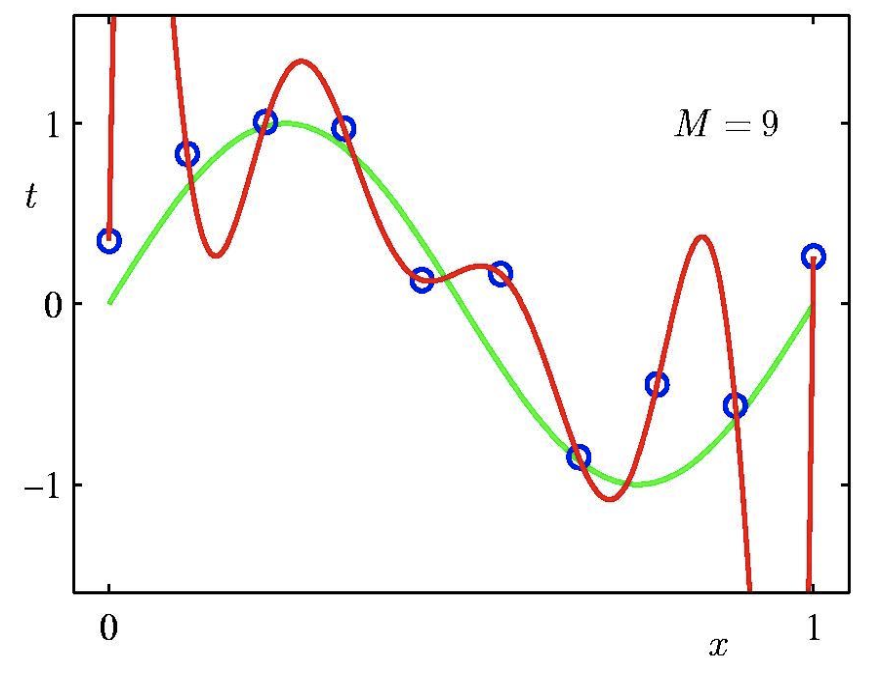
\includegraphics[width=\textwidth]{images/9st-order-polynomial.png}
        \caption{9st order polynomial}
    \end{subfigure}
\end{figure}

\hspace{-15pt}Notiamo che l'ultimo caso è molto più flessibile, ma potrebbe essere eccessivo. $E(w) = 0$ nei dati di training, diventa
un modello tropp complesso, scarsa rappresentazione della funzione vera (verde) (a causa del sovradattamento).\\\\
Capiamo dunque che il tradeoff della complessità è che:
\begin{itemize}
    \item Un modello troppo semplice: non fitta i dati in modo corretto \textbf{underfitting}
    \item Un modello troppo complesso: Altamente sensibile alle leggere perturbazioni dei dati \textbf{overfitting}
\end{itemize}
Vuoi scegliere la regolarizzazione per bilanciare i due casi attraverso il controllo della complessità del modello (intesa come flessibilità).
Considerando che la complessità non è dovuta al costo computazionale ma a misura della flessibilità del modello per adattarsi ai dati.

\subsection{Regularization}
Con la \textbf{regularization} possiamo controllare l'overfitting andando a pensalizzare la complessità delle funzioni con valori dei pesi grandi ($w$) (per ess.
verso il coefficiente restrigimento) o il numero dei parametri liberi ($w$ non uguale a zero). Tutto questo mentre si va a mantenere la flessibilità dello spazio
delle ipotesi.\\\\
\textbf{Occam (Ockham) razor}: "La spiegazione più semplice è più probabilmente quella corretta" o "Preferiscono l’ipotesi più semplice che si adatta ai dati".\\\\
Questo concetto fondamentale nel ML verrò ritrovato e lo "razzionalizzeremo" alla fine.

\begin{definition}
    Ridge regression o \textbf{tikhonov regularization}. La possinilità di aggiungere limitazioni alla somma di valori di $|w_j|$ favorendo modelli "scarsi" ess. con 
    meno termini dovuti ai pesi $w_j = 0$ (o vicino allo 0) (questo vuol dire modelli meno complessi).
    $$Loss(h_w) = \sum_{p=1}^{l}(y_p - h_w(x_p))^2 + \lambda||w||^2 \hspace{15pt} ||w||^2 = \sum_{i}w_i^2$$
    Termine di errorid dei dati + termine di regolarizzazione/penalità.
\end{definition}
\hspace{-15pt}Abbiamo che $\lambda$ è chiamato coefficiente di regolarizzazione (un parametro costante o un iperparamentro). L'effetto che abbiamo 
da questa regolarizzazione è il \textbf{decadimento del peso} (praticamente si aggiunge $2\lambda w$ al gradiante della peridita).
$$w_{new} = w + \eta \cdot \Delta w - w \lambda w$$
Per esempio con gradiante uguale a zero, esso decrementa il valore di ogni $w$ con una frazione della vecchia $w$.\\\\
Applicabilità generale (non sono per i polinomi): esempio possiamo controllare la complessità del modello salmente usando $\lambda$, senza conoscere
M come per i polinomi, o anche quando la complessità del modello non è conosciuta. \\
Notiamo il bilanciamento (compromesso) tra i due termini.Il termine relativo ai dati di errore di piccole dimensioni (minimizzare solo l'errore di addestramento) non
è sufficente per noi, vogliamo ance controllare la complessità del modello per contrallare l'\textbf{overfitting}, quindi introduciamo il secondo termine della minimizzazione.
Dall'altro canto possiamo eccedere perché troppo peso al secodo termine (alto valore $\lambda$) potra a focalizzare solo la minimizzazione (o principalemnte) sulla regolarizzazione,
quindi anche l'errore dei dati (primo termine) potrebbe aumetare molto, ovverso passare all'\textbf{underfitting}. Il compromesso è regolato dal valore di $\lambda$. 
\\\\Vediamo ora l'esempio fatto prima con un polinomio di nono grado applicaddo un $\lambda$
\begin{figure}[h!]
    \centering
    \begin{subfigure}{.3\textwidth}
        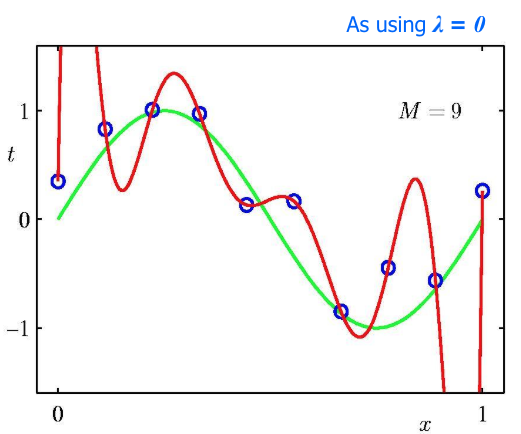
\includegraphics[width=\textwidth]{images/9-order-polynomial-with-lambda1.png}
        \caption{$\lambda = 0$}
    \end{subfigure}
    \begin{subfigure}{.3\textwidth}
        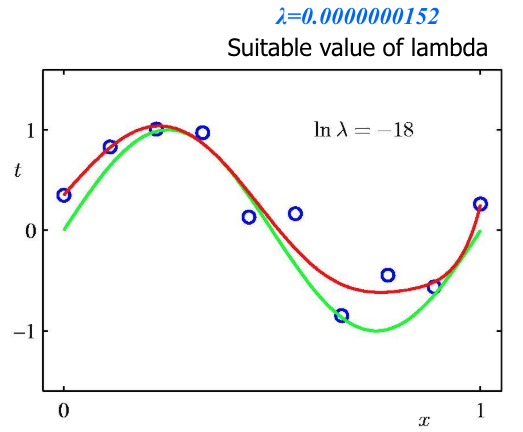
\includegraphics[width=\textwidth]{images/9-order-polynomial-with-lambda2.png}
        \caption{$\ln\lambda = -18$}
    \end{subfigure}
    \begin{subfigure}{.3\textwidth}
        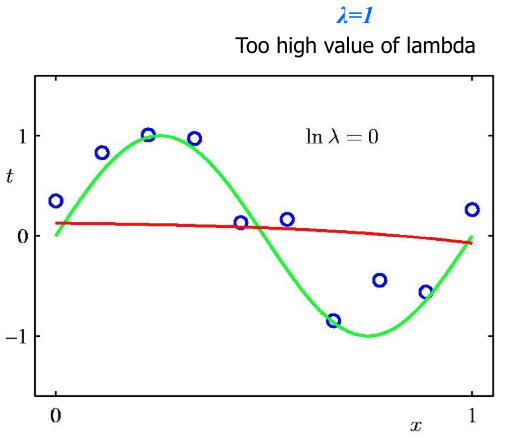
\includegraphics[width=\textwidth]{images/9-order-polynomial-with-lambda3.png}
        \caption{$\ln\lambda = 0 \Rightarrow \lambda = 1$}
    \end{subfigure}
\end{figure}
\begin{figure}[h!]
        \centering
    \begin{subfigure}{.42\textwidth}
        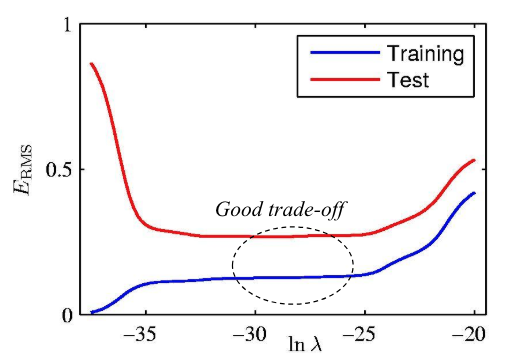
\includegraphics[width=\textwidth]{images/regularization.png}
        \caption{$\lambda$ basso = overfiting, $\lambda$ alto = underfitting}
    \end{subfigure}
    \begin{subfigure}{.42\textwidth}
        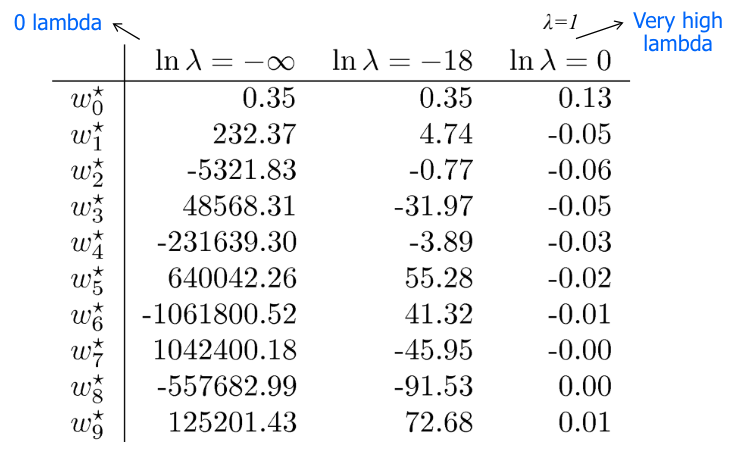
\includegraphics[width=\textwidth]{images/coefficente-polinomiale.png}
        \caption{Tabella coefficienti polinomiali}
    \end{subfigure}
\end{figure}
\subsubsection{Limitazioni di una funzione a base fissa}
Avente funzioni di base lungo ciascuno spazio di input di dimensioni n richeide un nunmero combinatorio di funzioni, 
esempio, un polinomio generale di ordine 3 usa tutte le combinazioni delle variabili di input dovute per produrre 
$x_1, x_2, x_2, x_3, \dots, x_1x_2,x_3$ etc $\to n^3$ (approssimazione al crescere di $n$).\\\\
I dati diventano sparsi in questo alto volume, quindi l'allomanre dei dati necessari per supportare il risultato
spesso cresce esponenzialmente con la dimensione. $\phi$ viene fissata prima di osservare i dati di allenamento. \\\\
In altri modelli, vedremo come possiamo farla franca con meno funzioni di base, andando a sceglierre questi usando i dati di training:
$\phi$ (in uno strato computazionale nascoso) dipende. In altri modelli il calcolo di inslusione (trasformazione dell'input)
è realizzato implicitamente attravero le funzioni del kernel e controllando la complessità del modello. Per esempio SVM.

\subsection{Classification}
Andiamo a ri-usare i modelli lineari, infatti gli stessi modelli possono essere usati per la \textbf{classificazione}, ci sono delle categorie target per esempio $0/1$ o $-1/+1$. In questo caso usiamo
un iperpiano ($wx$) assumento valori negativi o positivi. Sfruttiamo tali modelli per decidere se un punto x appartiene alla zona positiva o nogtiva 
dell'iperpiano (per classificarlo). Quindi vogliamo impostare $w$ (nel learning) per ottenere una buona precisione di classificazione.\\\\
Per per notazione di un input multidimensionale è come spiegato prima quindi, assumiamo una colonna vettore per $x$ e $w$, numero di dati $l$, dimensione
del vettore di input $n$, $y_p$ che è $d_p$ o $t_p$ (targets 0/1 o -1/+1 è la cosa nuova).
$$w^Tx + w_0 = w_0 + w_1x_1 + w_2 x_2 + \cdots + w_n x_n$$
Con $w_0$ che è un intercept, threshold, bias, offset ... Genericamente è convenzione includere la constante $x_0 = 1$ così si può riscrivere il tutto come
$$w^T x = x^T w \hspace{15pt} x^T = [1, x_1, x_2, \dots, x_n] \hspace{15pt} w^T = [w_0, w_1, w_2, \dots, w_n]$$ 
Vediamo ora la vista geometrica dell'iperpiano. Visto che $w^T x$ definisce un iperpiano abbiamo che
\begin{figure}[h!]
    \centering
    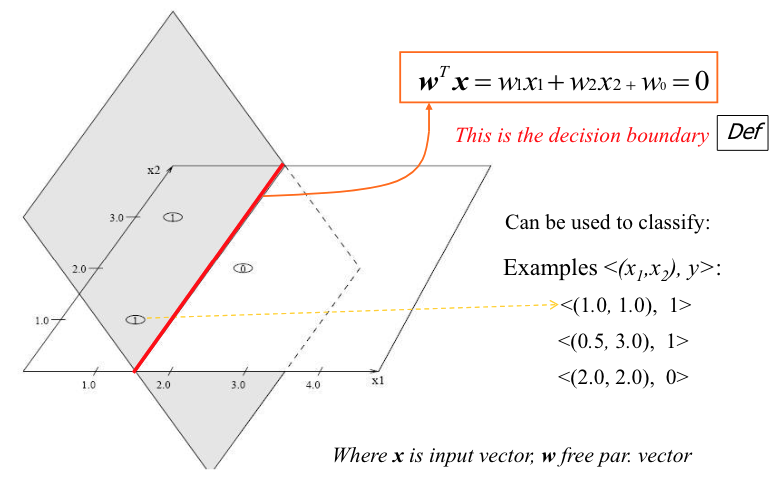
\includegraphics[width=0.45\textwidth]{images/iperpiano.png}
\end{figure}

\hspace{-15pt}Da questo possiamo anche vedere la vista geometrica della classificazione.
\begin{figure}[h!]
    \centering
    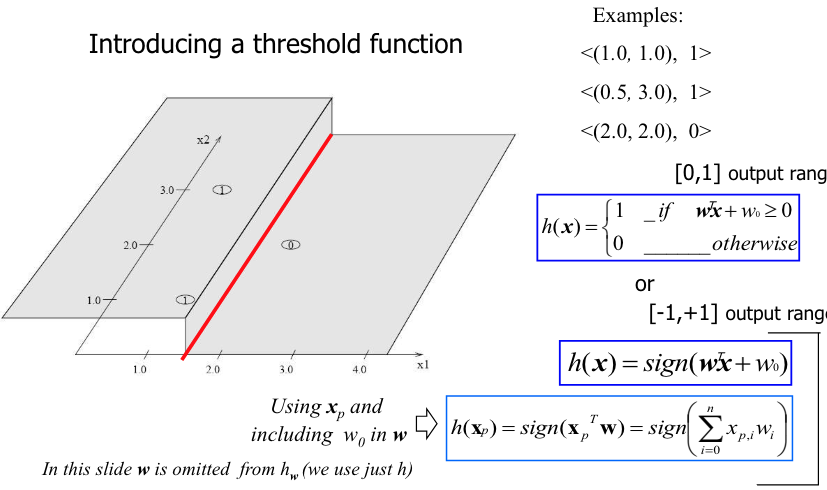
\includegraphics[width=0.45\textwidth]{images/geometric-classification.png}
\end{figure}
La classificazione può essere vista come un allocazione dello spazio di input nella regione di decisioni (es. 0/1). 2-dim spazioe di instance
$x=(x_1, x_2) \in R^2, f(x) = 0/1$ (o $-1/+1$) 
\begin{figure}[h!]
    \centering
    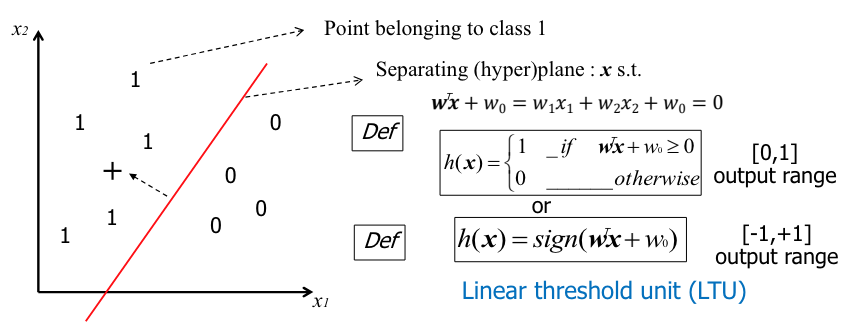
\includegraphics[width=0.5\textwidth]{images/classification-by-linear-dec-boundary.png}
\end{figure}
Notiamo che, dato una bias $w_0$, nella LTU diciamo che $h(x) = w^T x + w_0 \geq 0$ che è equivalente nel dire $h(x) = w^T x \geq -w_0$ con $-w_0$ abbiamo il valore "soglia".\\\\
Le due forme identificato la stessa zona positiva della classificazione, la seconda in particolare enfatizza il ruolo del bias come un valore soglia per "attivare" il +1 output del classifier.
\begin{example}
    Trovare h tale che dato $(x_1, x_2)$ retorni $0/-1$ per terremoti e $+1$ per una esplosione nucleare. Vediamo che l'algoritmo di learning trova questo confine di decisione:
    \begin{figure}[h!]
        \centering
        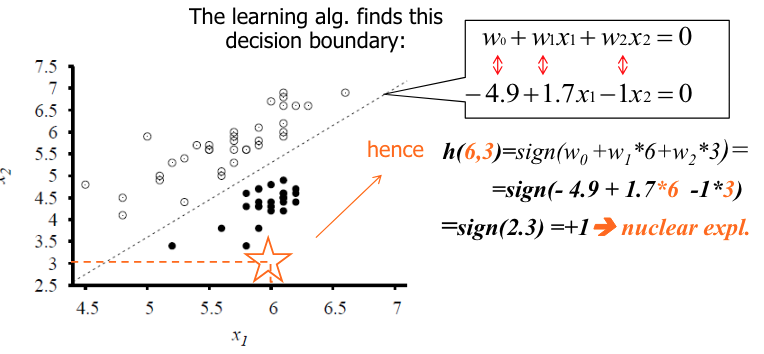
\includegraphics[width=0.6\textwidth]{images/esempio-classification.png}
    \end{figure}
    Dati sismici: $x_1$ magnitudo dell'onda corporea, $x_2$ magnitudo delle onde superficiali terremoti (bianco), esplosioni nucleari (nero).
\end{example}
\begin{example}
    Un altro esempio è quello dello spam. Trovare $h(mail) +1 $ per spam, e $-1$ per non-spam. Le carateristiche sono che $\phi(mail) = parole [0/1]$ o $frasi$ ("free money") $[0/1]$ o lunghezza [intero].
    Per esempio $\phi_k(x) = conain(word_k)$. Il peso $w$ contributo delle caratteristiche di input per la previsione, per esempio peso positivo per "denaro gratutito", negativo per ".edu". $x^Tw$ è la combinazione dei pesi.
    $h_w(x)$ fornisce la soglia per decidere se spam o non spam.
    $$h_w(x) = sign(\sum_{k}w_k \phi_k(x)) \:\:\:\: > 0 \to +1 = Spam$$  
\end{example}
\hspace{-15pt}Vediamo ora $\Delta w $ come correzione degli errori, regola di apprendimento.
$$\Delta w_i = \sum_{p=1}^{l}(y_p - x_p^T w) \cdot x_{p,i}$$
\begin{figure}[h!]
    \centering
    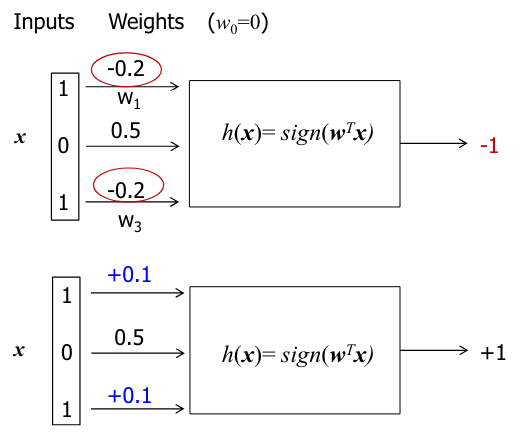
\includegraphics[width=0.5\textwidth]{images/delta-w-correzione-errore.png}
\end{figure}
Se classificato erroneamente (Perché il bersaglio è +1) $\to$ (1-(-???)) $\to$ delta positivo elevato per $w_1$ e $w_3$ $\to$ verranno aumenti
proporzionalmente (con età) a il delta, quindi valore positivo in questo caso (errore regola di correzione). Per esempio la parte rossa in figura.

\subsection{Learning algorithm}
Come per la regressione si possono applicare anche l'espansione in base lineare e Tikhonov, notare che (algoritmo di apprendimento) converte asintoticamente al MinLS e non
necessariamente al numero minimo di errori di classificazione. $[(\#ML)]$ se $w$ non vengono modificati per ottenere output corretti $(h_w(x_p) = d_p)$ otteniamo la rgola di aggiornamento per per \textbf{percettrone}
\begin{example}
    Vediamo l'esempio della congiunzone. Possiamo andarla a rappresentare tramite un modello lineare per esempio:
    $$h(x) = 
    \begin{cases}
        1 & if wx + w_0 \geq 0\\
        0 & otherwise
    \end{cases}
    $$
    La \textbf{congiunzione} avviene nel seguente modo: \\
    \begin{minipage}{.5\linewidth}
        4 var $x_1 \land x_w \land x_4 \Leftrightarrow y$
        \begin{itemize}
            \item $1x_1 + 1 x_2 + 0 x_3 + 1 x_4 > 2$
            \item $1x_1 + 1 x_2 + 0 x_3 + 1 x_4 \geq 2.5$
        \end{itemize}
        2 var: $x_1 \land x_2 \Leftrightarrow y$
        \begin{itemize}
            \item $1 x_1 + 1 x_2 > 1$
            \item $1 x_1 + 1 x_2 \geq 1.5$
        \end{itemize}
    \end{minipage}
    \hfill
    \begin{minipage}{.5\linewidth}
        \centering
        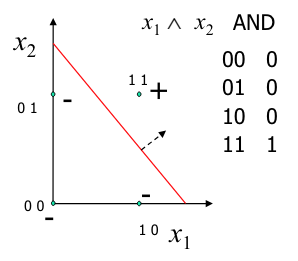
\includegraphics[width=0.7\linewidth]{images/esempio-congiunzione.png}
    \end{minipage}
\end{example}
\hspace{-15pt}In geometrica due insiemi di punti in un grafico bidimensionale sono \textbf{linearmente separabili} quando gli insiemi
di punti possono essere completamente separati da un'unica linea.
\begin{definition}
    In generale due gruppi sono detti \textbf{linearmente separabili} in uno spazio n-dimensionale se possono essere separati da un iperpiano di dimensione (n-1).
\end{definition}
\hspace{-15pt}Il confine decisionale lineare può fornire solo soluzioni esatte per insiemi di punti linearmente separabili.
\begin{example}
    Esempi di limiti decisionali non lineari. Ricordiamo che anche l'\textbf{espansione in base lineare} e la \textbf{regolaizzazione di Tikhonov} può anche essere applicato.
    \begin{figure}[h!]
        \centering
        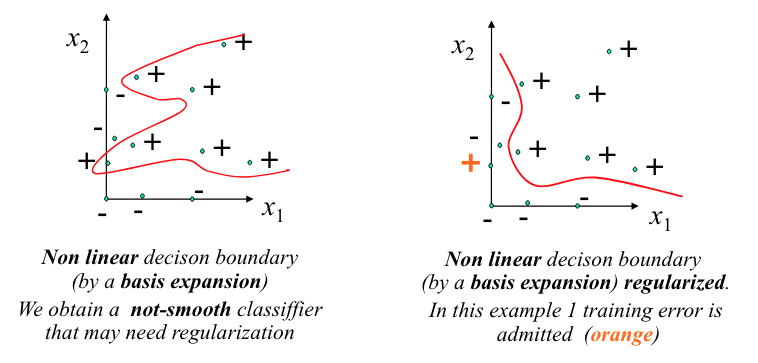
\includegraphics[width=0.7\textwidth]{images/esempio-non-linear-decision-boundary.png}
    \end{figure}
\end{example}
\hspace{-15pt}Ci sono anche altri modelli lineare per la classificazione:
\begin{itemize}
    \item Analisi discriminate lineare (anche mutliclasse)
    \item Regressione ligica. Nel quale $P(y|x)$ parte dalla modellazione della densità di classe come densità nota. Soglia leggera (continua, differenziabile) con una funzione logica.
    \item Reti neurali (NN) e SVM menzionate in precedenta: \textbf{modelli flessibili} includono l'approssimazione non lineare per entrambe le regressioni e classificazioni. [\#ML].
    \begin{itemize}
        \item Le NN utilizzano molte unità (simili a LTU) all'interno di diversi strati
        \item Apprendimento della rappresentazione delle funzionalità in ogni livello (concetto di deep learning)
        \item Approccio di discesa del gradiente per l'apprendimento.
    \end{itemize}
\end{itemize}
In conclusione i modelli linari sono degli aprocci di base ben fondati sia per la regressione che per la classificazione.
Sono un modo molto compatto per rappresentare la conoscenza, ma con un forte presupporto sulla relazione tra i dati. \\\\
Un algoritmo iterativo correzione degli errori (LMS) che esegue la ricerca in spazi di ipotesi continui (questa è òa base per molti altri approcci ML).\\\\
Una visione dei limiti degli approcci lineari e delle necessità di modelli ML più \textbf{flessibili} e relativi problemi sono un'estensione del modello lineare per compiti non lineari e 
un'introduzione al \textbf{controllo della complessità (regolaizzazione)}.